\documentclass[a4paper]{article}

\usepackage[margin=1in]{geometry}

\usepackage{mathtools}
\usepackage{derivative}
\usepackage{graphicx}
\usepackage{enumitem} % enumeration label options
\usepackage{amsfonts} % \mathbb, ...
\usepackage{amssymb} % \subsetneq, \nmid, ...
\usepackage{stmaryrd} % \mapsfrom
\usepackage{yhmath} % \widehat
\usepackage{tikz-cd}
\usepackage{amsthm}
\usepackage{dynkin-diagrams}

\setlength{\parindent}{0pt}

\newtheorem*{theorem}{Theorem}
\newtheorem*{lemma}{Lemma}
\newtheorem*{proposition}{Proposition}
\newtheorem*{corollary}{Corollary}
\newtheorem*{claim}{Claim}

\theoremstyle{definition}
\newtheorem*{definition}{Definition}
\newtheorem*{fact}{Fact}

\theoremstyle{remark}
\newtheorem*{example}{Example}
\newtheorem*{remark}{Remark}
\newtheorem*{exercise}{Exercise}

\DeclareMathOperator{\Hol}{Hol}
\DeclareMathOperator{\Sp}{Sp}
\DeclareMathOperator{\SO}{SO}
\DeclareMathOperator{\SL}{SL}
\DeclareMathOperator{\GL}{GL}
\DeclareMathOperator{\im}{im}
\DeclareMathOperator{\rad}{rad}
\DeclareMathOperator{\sgn}{sgn}
\DeclareMathOperator{\rank}{rank}

\newcommand{\id}{\mathrm{id}}
\newcommand{\dR}{\mathrm{dR}}
\newcommand{\FS}{\mathrm{FS}}

\newcommand{\E}{\mathcal{E}}
\newcommand{\U}{\mathcal{U}}
\renewcommand{\u}{\mathfrak{u}}
\newcommand{\m}{\mathfrak{m}}
\newcommand{\CP}{\mathbb{CP}}
\newcommand{\F}{\mathbb{F}}
\renewcommand{\H}{\mathbb{H}}
\renewcommand{\O}{\mathbb{O}}
\renewcommand{\P}{\mathbb{P}}
\newcommand{\A}{\mathbb{A}}
\newcommand{\N}{\mathbb{N}}
\newcommand{\Z}{\mathbb{Z}}
\newcommand{\Q}{\mathbb{Q}}
\newcommand{\R}{\mathbb{R}}
\newcommand{\C}{\mathbb{C}}

\title{Topics in Geometry (LSGNT) - Notes and Exercises}
\author{Calum Crossley}
\date{2023-2024}

\begin{document}

\maketitle

\section{Spec and Proj - Ed Segal}

% TODO: Add notes for this maybe?

\subsection*{Exercise solutions}

\begin{enumerate}

\item
\begin{enumerate}[label=(\alph*)]

\item 
A decomposition $V=V_1\cup V_2$ into subvarieties (Zariski
closed sets) $V_1$ and $V_2$ is the same thing as a pair of
disjoint Zariski open sets $V\setminus V_1$ and
$V\setminus V_2$. The decomposition is non-trivial iff the open
sets are non-empty.

\item
If $fg=0$ in $\C[V]$ then $V=V(f)\cup V(g)$, so irreducibility
implies one of $V(f)$ or $V(g)$ is $V$, meaning one of $f$ or
$g$ is zero. Hence $\C[V]$ is an integral domain if $V$ is
irreducible.

If $V=V_1\cup V_2$ and $V_i\ne V$ then some polynomial
$f_i$ vanishes on $V_i$ but not $V$, otherwise the equations
defining $V_i$ would include all of $V$. Then $f_1f_2$ vanishes
on $V_1\cup V_2=V$, so $\C[V]$ has zero-divisors.

\end{enumerate}

\item
\begin{enumerate}[label=(\alph*)]

\item 
Let $f$ be a non-constant polynomial with no roots over a non-algebraically
closed field, such as $x^2+1$ over $\R$. Then $V(f)=\emptyset$ so
$I_{V(f)}=(1)$, but $1\notin\rad(f)$ as $f$ is non-constant.

\item
Over $\F_p$ affine space $\A^n$ has finitely many points, so $I_{\A^n}$ consists
of the polynomials vanishing at these points, including for example
$\prod_{a_1\in\F_p}(x_1-a_1)=x_1^p-x_1$. We have
\begin{align*}
    I_{\A^n(\F_p)}
        &= \bigcap_{a_1,\ldots,a_n\in\F_p}(x_1-a_1,\ldots,x_n-a_n) \\
        &= \bigcap_{a_2,\ldots,a_n\in\F_p}(x_1^p-x_1,x_2-a_2,\ldots,x_n-a_n) \\
        &= (x_1^p-x_1,\ldots,x_n^p-x_n).
\end{align*}

\end{enumerate}

\item
Consider the affine variety $X=V(x_{n+1}f-1)\subseteq\A^{n+1}$. We have a
morphism $X\to\A^n\setminus V(f)$ by projection:
$(a_1,\ldots,a_{n+1})\mapsto(a_1,\ldots,a_n)$, since
$a_{n+1}f(a_1,\ldots,a_n)=1$ implies $f(a_1,\ldots,a_n)\ne0$. This has an
inverse given by $(a_1,\ldots,a_n)\mapsto(a_1,\ldots,a_n,1/f(a_1,\ldots,a_n))$,
which is also regular.

\item
Suppose $V\subseteq\A^n$ and $W\subseteq\A^m$, corresponding to quotient maps
$\C[x_1,\ldots,x_n]\to\C[V]$ and $\C[y_1,\ldots,y_m]\to\C[W]$. Choose a
lift of $\C[W]\to\C[V]$ and let $f_1,\ldots,f_m\in\C[x_1,\ldots,x_n]$
be the images of $y_1,\ldots,y_m$, as in the following diagram.
\begin{equation*}
\begin{tikzcd}[column sep=huge]
    &\C[W] \ar[r] &\C[V] \\
    &\C[y_1,\ldots,y_m] \ar[u,two heads] \ar[r,dashed,"f_1{,}\ldots{,}f_m"]
    &\C[x_1,\ldots,x_n] \ar[u,two heads]
\end{tikzcd}
\end{equation*}
Then $(x_1,\ldots,x_n)\mapsto(f_1,\ldots,f_m)$ is a morphism $\A^n\to\A^m$, and
since $I_W$ maps to $I_V$ in the diagram, it restricts to a morphism $V\to W$.
Moreover the pullback $\C[V]\to\C[W]$ given by composition with this map
precisely corresponds to substituting $f_1,\ldots,f_m$ for $y_1,\ldots,y_m$, so
from the diagram we recover the original homomorphism $\C[W]\to\C[V]$.

\item
If $\varphi:\C[V]\to\C[x]/(x^2)$ we have $\C[V]\to\C[x]/(x^2)\to\C[x]/(x)=\C$,
and the kernel of this map is a maximal ideal
$\m_p=\varphi^{-1}((x))\subseteq\C[V]$ corresponding to a point $p\in V$.
Moreover $\m_p/\m_p^2$ maps to $(x)/(x^2)=\C\cdot x$, giving an element of the
dual $(\m_p/\m_p^2)^\vee$ of $\m_p/\m_p^2$ considered as a
$\C[V]/\m_p=\C$-vector space.

\textbf{Claim 1:}
The data of a maximal ideal $\m_p\subseteq\C[V]$ and a functional
$v\in(\m_p/\m_p^2)^\vee$ determines a unique homomorphism $\C[V]\to\C[x]/(x^2)$
respecting the above construction.

\textbf{Proof:}
Define $\C[V]\to\C[x]/(x^2)$ by $f\mapsto f(p)+v(f-f(p))x$. This is clearly
$\C$-linear, and respects products since
\begin{equation*}
    fg-f(p)g(p) \equiv f(p)(g-g(p)) + g(p)(f-f(p)) \mod \m_p^2;
\end{equation*}
the difference being $(f-f(p))(g-g(p))$. By construction the preimage of $(x)$
is $\m_p$, and the induced map $\m_p/\m_p^2\to(x)/(x^2)=\C\cdot x$ is indeed
given by $v$.

\textbf{Claim 2:}
The space $(\m_p/\m_p^2)^\vee$ is canonically identified with the tangent space
to $V$ at $p$.

\textbf{Proof:}
Inuitively, elements of $(\m_p/\m_p^2)^\vee$ are functionals insensitive to
second order vanishing, which are first order differential operators;
differentiation along tangent vectors. Suppose
$V=V(f_1,\ldots,f_r)\subseteq\A^n$. Then the tangent space to $V$ at $p$ should
be given by
\begin{equation*}
    T_pV = \left\{(v_1,\ldots,v_n)\in\C^n
        : v_1\pdv{f_i}{x_1}(p)+\cdots+v_n\pdv{f_i}{x_n}(p)=0
        \text{ for $i=1,\ldots,r$}\right\}.
\end{equation*}
We define $\psi:(\m_p/\m_p^2)^\vee\to T_pV$ by
$v\mapsto(v(x_1-p_1),\ldots,v(x_n-p_n))$; evaluating the operator on
coordinates. This is well-defined since
\begin{equation*}
    (x_1-p_1)\pdv{f_i}{x_1}(p) + \cdots + (x_n-p_n)\pdv{f_i}{x_n}(p)
        \equiv f_i \mod \m_p^2,
\end{equation*}
and $f_i=0$ in $\C[V]$. It has an inverse given by
\begin{equation*}
    (v_1,\ldots,v_n) \mapsto
        \left(f\mapsto v_1\pdv{f}{x_1}(p)+\cdots+v_n\pdv{f}{x_n}(p)\right),
\end{equation*}
which is well-defined since elements of $\m_p^2$ map to zero by the product
rule, and multiples of $f_1,\ldots,f_r$ map to zero by the product rule and the
fact that $(v_1,\ldots,v_n)\in T_pV$. That this is indeed an inverse follows
from the fact that
\begin{equation*}
    (x_1-p_1)\pdv{f}{x_1}(p) + \cdots + (x_n-p_n)\pdv{f}{x_n}(p)
        \equiv f \mod \m_p^2.
\end{equation*}

\item
The corresponding homomorphism of coordinate rings $\C[x,y]/(y^2-x^3)\to\C[t]$
given by $x\mapsto t^2$, $y\mapsto t^3$ is not an isomorphism, since
$\C[t^2,t^3]\subsetneq\C[t]$.

However we have a set-theoretic inverse:
\begin{equation*}
    (x,y)\mapsto\begin{dcases*}
        x/y & if $y\ne0$ \\
        0 & otherwise.
    \end{dcases*}
\end{equation*}
Adjoining a point at infinity to both curves we get compact Hausdorff spaces in
the complex topology, so this inverse is even continuous with respect to the
complex topology.

\item
For $U_0\cap U_1$ we have $[1,x_1,x_2]=[1/x_1,1,x_2/x_1]$, giving
$(x_1,x_2)\mapsto(1/x_1,x_2/x_1)$.

For $U_0\cap U_2$ we have $[1,x_1,x_2]=[1/x_2,x_1/x_2,1]$, giving
$(x_1,x_2)\mapsto(1/x_2,x_1/x_2)$.

For $U_1\cap U_2$ we have $[x_0,1,x_2]=[x_0/x_2,1/x_2,1]$, giving
$(x_0,x_2)\mapsto(x_0/x_2,1/x_2)$.

\item
Suppose $f\in\C[x_1,\ldots,x_n]$ defines a hypersurface $V=V(f)\subseteq\A^n$.
We obtain a homogeneous polynomial $\hat f\in\C[x_1,\ldots,x_{n+1}]$ by
\begin{equation*}
    \hat f = x_{n+1}^{\deg f}\cdot f(x_1/x_{n+1},\ldots,x_n/x_{n+1}),
\end{equation*}
giving a projective hypersurface in $\P^n$ whose intersection with the affine
part $x_{n+1}\ne0$ is $V(f)$. It is in fact the closure of this affine part in
$\P^n$, since substituting $x_{n+1}=1$ and applying this process to a
homogeneous polynomial recovers the original polynomial up to a multiple of
$x_{n+1}$. When the codimension is higher homogenizing the generators of the
defining ideal like this is insufficient to cut out the projective closure; one
must homogenize all elements of the vanishing ideal. For example homogenizing
the generators of $V(x_1-x_2^2,x_1-x_3^3)$ gives
$V(x_1x_4-x_2^2,x_1x_4^2-x_3^3)$, whose points at infinity are given by

\item
\begin{enumerate}[label=(\alph*)]

\item 
Define a map $\P^1\to C$ by $[s:t]\mapsto[s^2:t^2:st]$. Now $xy=z^2$ implies
$[y:z]=[z:x]$ when both are defined, so $[x:y:z]\mapsto[y:z]$ and
$[x:y:z]\mapsto[z:x]$ glue to give an inverse $C\to\P^1$.

\item
Matrices of rank 1 are non-zero, and the rank is preserved by non-zero scalar
multiplication. Non-zero traceless $2\times2$ matrices are parametrized up to
scale by $\P^2$ as follows:
\begin{equation*}
    [x:y:z] \mapsto \begin{pmatrix}
        z & -x \\ y & -z
    \end{pmatrix},
\end{equation*}
and the rank is 1 iff the determinant $xy-z^2$ vanishes. Hence $C$ parametrizes
rank 1 traceless $2\times2$ matrices up to scale. From (a) we also get a
parametrization by $\P^1$:
\begin{equation*}
    [s:t] \mapsto \begin{pmatrix}
        st & -s^2 \\ t^2 & -st
    \end{pmatrix}.
\end{equation*}

\item
Over $\C$ the quadratic forms are determined up to equivalence by rank, so
replacing $xy-z^2$ by a non-degenerate quadratic form results in a curve
isomorphic to $C\cong\P^1$. A quadratic form of rank 2 results in a curve
isomorphic to $V(xy)$; two lines, and a quadratic form of rank 1 results in a
curve isomorphic to $V(x^2)$; one line (or a scheme-theoretic double line).

Different quadratic forms correspond to different special matrix forms as in
(b), for example
\begin{equation*}
    x^2 + y^2 = \det\begin{pmatrix}
        x & -y \\
        y & x
    \end{pmatrix}
\end{equation*}
and
\begin{equation*}
    xw - yz = \det\begin{pmatrix}
        x & y \\ z & w
    \end{pmatrix}.
\end{equation*}
The latter gives the Segre embedding $\P^1\times\P^1\to\P^3$,
$(X_1:X_2,Y_1:Y_2)\mapsto(X_1Y_1:X_1Y_2:X_2Y_1:X_2Y_2)$, whose image is
$V(XW-YZ)$.

\end{enumerate}

\item
\begin{enumerate}[label=(\alph*)]

\item
For $\epsilon\ne0$ we have $V_\epsilon\cong\A^1\setminus\{0\}$ via
$z\mapsto(z,\epsilon/z)$, which is
$(re^{i\theta},\epsilon r^{-1}e^{-i\theta})$
in polar coordinates. This forms a cylinder joining up the two real arcs
$\theta=0$ and $\theta=\pi$, with $(x,y)$ connecting to $(-x,-y)$ on the circle
$r=|x|$.

% TODO: picture

If we follow the circles $r=c$ for constant $c$ as $\epsilon\to0$ we get the
circles around the origin of the $x$-plane in $xy=0$. Similarly the circles
$r=c\epsilon$ converge to the circles around the origin of the $y$-plane.
Meanwhile the circle $r=\sqrt{|\epsilon|}$ contracts to the origin, so the
cylinder is pinched into two planes / discs connected at the origin.

\item % TODO

\end{enumerate}

\end{enumerate}

\section{Poincar\'e duality - Steven Sivek}

Recommended source: Bott \& Tu, Differential Forms in Algebraic Topology.

\subsection*{Rough idea}

Take a (smooth, oriented) manifold $M^n$. Compact (smooth, oriented) submanifolds
$X^k,Y^{n-k}\subseteq M$ intersect \emph{transversely} at $p\in X\cap Y$ if we
have
\begin{equation*}
    T_pX\oplus T_pY = \pm T_pM,
\end{equation*}
where the sign matches the orientation on the LHS induced from $X$ and $Y$ with
the orientation of $M$. Write $\sgn(p)$ for this sign, and define the
\emph{intersection number}
\begin{equation*}
    i(X,Y) = \sum_{p\in X\cap Y}\sgn(p).
\end{equation*}

\begin{claim}
    This only depends on $[X]\in H_k(M)$, $[Y]\in H_{n-k}(M)$. Hence we get a
    bilinear form
    \begin{equation*}
        i:\frac{H_k(M)}{\text{torsion}}
            \otimes\frac{H_{n-k}(M)}{\text{torsion}}\to\Z.
    \end{equation*}
    (We can mod out by torsion since $\Z$ is torsion-free.)
\end{claim}

\begin{theorem}[Poincar\'e duality]
    This form is non-degenerate; if $i(X,Y)=0$ for all $Y$ then $X=0$.
\end{theorem}

\begin{corollary}
    We have $\rank H_k(M)=\rank H_{n-k}(M)$ for each $k$.
\end{corollary}

Suppose $\dim M=2m$. We get a pairing on $H_m(M)/\text{torsion}$, and this is
symmetric or anti-symmetric if $m$ is even or odd respectively (think about the
orientation of $T_pX\oplus T_pY$ vs. $T_pY\oplus T_pX$). Then Poincar\'e duality
says that this pairing is \emph{uni-modular}; the matrix representing it in an
integral basis has determinant $\pm1$.

The algebraic structure $(H_m(M),i)$ is an invariant of $M$. When $\dim M=4$ we
define the \emph{signature} $\sigma(M)$ to be the signature of this bilinear
form.

\begin{theorem}
    $\sigma(M)$ is a complete bordism invariant of oriented 4-manifolds.
\end{theorem}

\begin{theorem}[Donaldson]
    If $M^4$ is smooth, and $i_M$ is negative-definite, then $i_M$ is
    diagonalizable over $\Z$; given by $-I$ in some integral basis for $H_2(M)$.
\end{theorem}

\begin{theorem}[Freedman]
    There exists a topological manifold $M^4$ with $i_M=E_8$, which is
    negative-definite but not diagonalizable over $\Z$. Hence $M$ has no smooth
    structure.
\end{theorem}

(The form $E_8$ is defined on $\Z^8$ by the adjacency matrix for the Dynkin
diagram \dynkin{E}{8}.)

\subsection*{de Rham cohomology}

\begin{definition}
    A \emph{$k$-form} on $M$ is a section of $\Lambda^kT^*M$. That is, at every
    point a multilinear alternating form
    $\alpha_p:\underbrace{T_pM\otimes\cdots\otimes T_pM}_{\text{$k$ times}}\to\R$.
\end{definition}

The space $\Omega^k(M)$ of $k$-forms has extra structure:
\begin{itemize}
    \item Wedge product $\wedge:\Omega^k(M)\otimes\Omega^l(M)\to\Omega^{k+l}(M)$
    \item Exterior derivative $d:\Omega^k(M)\to\Omega^{k+1}(M)$
\end{itemize}
satisfying
\begin{itemize}
    \item $\alpha\wedge\beta=(-1)^{|\alpha|\cdot|\beta|}\beta\wedge\alpha$
    \item $d(\alpha\wedge\beta)
        = d\alpha\wedge\beta+(-1)^{|\alpha|}\alpha\wedge d\beta$ (Leibniz rule)
    \item $d^2=0$.
\end{itemize}
This is the structure of a differential graded algebra, which is nice.

On $\R^n$, these operations are defined as follows:
\begin{itemize}
    \item $\Omega^k(\R^n)=\R\cdot\{fdx_{i_1}\wedge\cdots\wedge dx_{i_k}\}$,
        where $dx_i(\pdv{}{x_j})=\delta_{ij}$.

    \item $(fdx_{i_1}\wedge\cdots\wedge dx_{i_k})
                \wedge(gdx_{j_1}\wedge\cdots\wedge dx_{j_l})
            = fgdx_{i_1}\wedge\cdots\wedge dx_{i_k}
                \wedge dx_{j_1}\wedge\cdots\wedge dx_{j_l}$.

    \item $d(fdx_{i_1}\wedge\cdots\wedge dx_{i_k})
        = (\sum_i\pdv{f}{x_i}dx_i)\wedge dx_{i_1}\wedge\cdots\wedge dx_{i_k}$.
\end{itemize}
The general case is defined by patching these together from local coordinate
charts.

\begin{definition}
    A $k$-form $\alpha$ is \emph{closed} if $d\alpha=0$, and \emph{exact} if
    $\alpha=d\beta$ for some $(k-1)$-form $\beta$.

    The \emph{de Rham cohomology} is then
    \begin{equation*}
        H^k_\dR(M)
            = \{\text{closed $k$-forms}\}/\{\text{exact $k$-forms}\}
            = \ker d/\im d.
    \end{equation*}
\end{definition}

\begin{example}
    $\alpha\in\Omega^0(M)$ is a function, and locally
    $d\alpha=\sum_i\pdv{\alpha}{x_i}dx_i$, so $d\alpha=0$ iff $\alpha$ is
    locally constant. Hence $H^0_\dR(M)=\R$ if $M$ is connected.
\end{example}

\begin{example}
    If $k>\dim M$ then $\Omega^k(M)=0$ since $\Lambda^kT_pM=0$. Hence
    $H^k_\dR(M)=0$.
\end{example}

\begin{example}
    What is $H^1_\dR(\R)$? $\Omega^1(\R)=\{fdx:f:\R\to\R\}$ are all closed from
    above. Exact 1-forms are given by $dF=F'(x)dx$ for $F:\R\to\R$. Such an $F$
    with $dF=fdx$ always exists by the FTC, via
    \begin{equation*}
        F(x) = \int_0^xf(t)dt.
    \end{equation*}
    Hence $H^1_\dR(\R)=0$.
\end{example}

\begin{remark}
    By the Leibniz rule, the wedge product descends to cohomology, making
    $H^*_\dR(M)$ a graded-commutative $\R$-algebra.
\end{remark}

\begin{theorem}[Stokes' theorem]
    If $X^k\subseteq M^n$ is a compact submanifold with boundary, and
    $\alpha\in\Omega^{k-1}(M)$, we have
    \begin{equation*}
        \int_Xd\alpha = \int_{\partial X}\alpha.
    \end{equation*}
\end{theorem}

(Integration of forms is extended from $\R^n$ by patching.)

\begin{exercise}
    Show that there is a bilinear pairing
    \begin{equation*}
        H_k(M;\R)\otimes H^k_\dR(M)\to\R
    \end{equation*}
    given by
    \begin{equation*}
        [X^k]\otimes[\alpha]\mapsto\int_X\alpha.
    \end{equation*}
    (You may use a theorem of Thom, which states that after multiplying by a
    positive integer, any singular homology class of a manifold may be
    represented by a compact submanifold.)
\end{exercise}

\begin{proof}[Solution]
    For a homology class of the form $\frac{1}{n}[X^k]$ we define the image as
    \begin{equation*}
        \frac{1}{n}\int_X\alpha.
    \end{equation*}
    By the theorem of Thom on representability of multiples of homology classes
    this gives an output for all elementary tensors. It is well-defined, for if
    $\frac{1}{n}[X^k]=\frac{1}{m}[Y^k]$ then their difference is the boundary of
    some $(k+1)$-chain $c$, so
    \begin{equation*}
        \frac{1}{n}\int_X\alpha - \frac{1}{m}\int_Y\alpha
            = \int_{\partial c}\alpha
            = \int_cd\alpha
    \end{equation*}
    by Stokes' theorem, which is zero since $d\alpha=0$.
\end{proof}

\begin{lemma}[Poincar\'e lemma]
    \begin{equation*}
        H^k_\dR(\R^n) = \begin{dcases*}
            \R & $k=0$ \\
            0 & otherwise.
        \end{dcases*}
    \end{equation*}
\end{lemma}

\begin{proof}
    We induct on $n$. Assume $k>0$, and that all closed $k$-forms on $\R^n$ are
    exact. Consider a closed form $\omega\in\Omega^k(\R^{n+1})$. Taking
    coordinates $(x,t)$ on $\R^{n+1}=\R^n_x\times\R_t$, we may write
    $\omega=\alpha_t+dt\wedge\beta_t$ where $\alpha_t\in\Omega^k(\R^n)$ and
    $\beta_t\in\Omega^{k-1}(\R^n)$ for each $t$. Define
    $\eta_t=\int_0^t\beta_sds$, so that $\odv{}{t}\eta_t=\beta_t$. We have
    \begin{align*}
        d\eta_t
            &= d_x\eta_t + dt\wedge\odv{}{t}\eta_t \\
            &= d_x\eta_t + dt\wedge\beta_t,
    \end{align*}
    so $\omega-d\eta_t=\alpha_t-d_x\eta_t$. The LHS is closed, so
    $\alpha_t-d_x\eta_t$ is a closed form on $\R^n\times\R$, and in particular
    must be constant in $t$, given by some form in $\Omega^k(\R^n)$ which is
    exact by induction. Say $\alpha_t-d_x\eta_t=d_x\xi$, where
    $\xi\in\Omega^{k-1}(\R^n)$. Then $\omega=d\eta_t+d\xi$ is exact, where we
    pull back $\xi$ to $\R^n\times\R$ as a constant in $t$.
\end{proof}

There is an important variant of de Rham cohomology:
\begin{equation*}
    \Omega^k_c(M) = \{\text{compactly supported $k$-forms}\}
\end{equation*}
retains the differential graded algebra structure, and gives rise to compactly
supported (de Rham) cohomology
\begin{equation*}
    H^k_c(M) = \frac{\ker(d:\Omega^k_c(M)\to\Omega^{k+1}_c(M))}
        {\im(\Omega^{k-1}_c(M)\to\Omega^k_c(M))}.
\end{equation*}

\begin{remark}
    If $M$ is compact, then $\Omega^k_c(M)=\Omega^k(M)$ and
    $H^k_\dR(M)=H^k_c(M)$.
\end{remark}

\begin{example}
    $\ker(d:\Omega^0_c(\R^n)\to\Omega^1_c(\R^n))
    =\{\text{constant compactly supported functions}\}=0$, so $H^0_c(\R^n)=0$.
\end{example}

\begin{exercise}
    Prove $\alpha\in\Omega^1_c(\R)$ is exact iff $\int_\R\alpha=0$. Conclude
    that $H^1_c(\R)\cong\R$.
\end{exercise}

\begin{proof}[Solution]
    If $\alpha=df$ then $\int_\R\alpha=\int_\R df=0$ by Stokes' theorem.
    Conversely, if $\int_\R\alpha=0$ then the function
    \begin{equation*}
        f(t)=\int_{(-\infty,t)}\alpha
    \end{equation*}
    is zero for $t$ past the support of $\alpha$, as well as for $t$ preceding
    the support of $\alpha$, so $f\in\Omega^0_c(\R)$. By construction
    $\alpha=df$. This shows that integration gives an injection
    $H^1_c(\R)\to\R$, which is non-zero by the existence of bump functions, and
    therefore gives an isomorphism $H^1_c(\R)\cong\R$.
\end{proof}

\begin{lemma}[Poincar\'e lemma, pt 2]
    \begin{equation*}
        H^k_c(\R^n) = \begin{dcases*}
            \R & $k=n$ \\
            0 & otherwise.
        \end{dcases*}
    \end{equation*}
\end{lemma}

\subsection*{Poincar\'e duality}

\begin{theorem}[Poincar\'e duality]
    There is a perfect pairing
    \begin{align*}
        H^k_\dR(M)&\otimes H^{n-k}_c(M) \to \R \\
        [\alpha]&\otimes[\beta] \mapsto \int_M\alpha\wedge\beta.
    \end{align*}
    Equivalently, we have an isomorphism
    \begin{align*}
        H^k_\dR(M) &\to H^{n-k}_c(M)^* \\
        [\alpha] &\mapsto \int_M\alpha\wedge(-).
    \end{align*}
\end{theorem}

\begin{proof}[Proof sketch]
    Take a good cover of $M$; an open cover $\U=\{U_i\}$ such that
    finite intersections of the $U_i$ are contractible (or just discs). Induct
    on $|\U|$.
    \begin{itemize}
        \item $|\U|=1$: $M=\R^n$ so we use the Poincar\'e lemma; it is easy to
            check that the pairing is non-zero.

        \item Inductive step: Write $U=U_1\cup\cdots\cup U_{n-1}$, $V=U_n$, and
            look at the Mayer-Vietoris sequences for $M=U\cup V$ in both
            cohomologies. There are natural comparison maps, which are
            isomorphisms by induction on all terms but the $M$ terms. By the
            five lemma they must also be isomorphisms on $M$.
    \end{itemize}
\end{proof}

There is a version of Poincar\'e duality for homology as well. Composing
\begin{equation*}
    \int : H_k(M;\R) \to H^k_\dR(M)^*
\end{equation*}
with the isomorphism $H^k_\dR(M)^*\cong H^{n-k}_c(M)$ gives
\begin{align*}
    \eta : H_k(M;\R) &\to H^{n-k}_c(M) \\
    [X] &\mapsto [\eta_X]
\end{align*}
satisfying $\int_X\alpha=\int_M\alpha\wedge\eta_X$. The class $[\eta_X]$ is
called the Poincar\'e dual of the submanifold $X$.

\begin{theorem}[Poincar\'e duality]
    $\eta:H_k(M;\R)\to H^{n-k}_c(M)$ is an isomorphism.
\end{theorem}

When $k=n-1$, we have an explicit construction for $\eta_X$ as follows:
$X^k\subseteq M^n$ has a tubular neighbourhood $N(X)\cong X\times[-1,1]_t$. (The
normal bundle is trivial since the codimension is 1 and everything is
orientable.) Define $\eta_X\in\Omega^1_c(M)$ by
\begin{equation*}
    (\eta_X)_p = \begin{dcases*}
        \phi(t)dt & $p=(x,t)\in N(X)$ \\
        0 & otherwise
    \end{dcases*}
\end{equation*}
where $\phi(t)$ is a bump function supported on $[-1,1]$ with total integral 1.
Then
\begin{itemize}
    \item $d\eta_X=0$ since $d(\phi(t)dt)=\phi'(t)d^2t=0$, so
        $[\eta_X]\in H^1_c(X)$ is well-defined.

    \item $\int_X\alpha=\int_{X\times[-1,1]}\alpha\wedge\phi(t)dt$ by Fubini,
        and this latter integral is just $\int_M\alpha\wedge\eta_X$.
\end{itemize}
Hence $[\eta_X]$ is the Poincar\'e dual for $X$.

The same idea works whenever the submanifold has a trivial normal bundle, but
there are complications for the general case.

\begin{exercise}
    Show that if $Y^1$ is transverse to $X^{n-1}$ in $M^n$, then
    \begin{equation*}
        \int_Y\eta_X = i(X,Y)
    \end{equation*}
    computes the intersection number.

    Hint: Work in explicit coordinates near $p\in X\cap Y$, and use the above
    construction of $\eta_X$.
\end{exercise}

\begin{proof}[Solution]
    The intersection $X\cap Y$ is a discrete and hence finite subset of $Y$.
    We can therefore take a small enough tubular neighbourhood of $X$ such that
    near each $p\in X\cap Y$, the component of $Y$ in this neighbourhood is parametrised as
    $(x(t),t)\in X\times[-1,1]\cong N(X)$. The integral $\int_Y\eta_X$ splits
    up as a sum over these components, and the integral for the component is
    \begin{equation*}
        \int_{\mp1}^{\pm1}\phi(t)dt = \pm1
    \end{equation*}
    depending on whether the orientation of $Y$ agrees with the positive
    direction in $t$ or not, since the pullback of $\eta_X=\phi(t)dt$ along
    $t\mapsto(y(t),t)$ is again $\phi(t)dt$. This is precisely the definition
    of $\sgn(p)$, so summing up gives
    \begin{equation*}
        \int_Y\eta_X = i(X,Y).
    \end{equation*}
\end{proof}

Since $\int_Y\eta_X=\int_M\eta_X\wedge\eta_Y$, we get
\begin{equation*}
    i(X,Y) = \int_M\eta_X\wedge\eta_Y.
\end{equation*}
Hence the Poincar\'e duality isomorphism $H_k(M;\R)\to H^{n-k}_c(M)$ identifies
the intersection form (cap product) on $H_*(M;\R)$ with the wedge product on
$H^*_c(M)$. It is an isomorphism of graded-commutative $\R$-algebras.

\section{Complex manifolds and the K\"ahler condition \\ - Lorenzo Foscolo}

\subsection*{Notes}

\subsubsection*{Almost-Hermitian geometry}

We have three geometric subgroups of $\GL(2n,\R)$;
\begin{itemize}
    \item $\GL(n,\C)$, which is the subgroup preserving the map
        $J_0:\R^{2n}\to\R^{2n}$ given by multiplication by $i$ under the
        identification $\R^{2n}\cong\C^n$, satisfying $J_0^2=-1$.

    \item $\Sp(2n,\R)$, which is the subgroup preserving the standard
        non-degenerate 2-form $\omega_0=dx_1\wedge dy_1+\cdots+dx_n\wedge dy_n$
        in coordinates $(x_1,y_1,\ldots,x_n,y_n)$.

    \item $\SO(2n)$, which is the subgroup preserving the standard Riemannian
        metric $g_0=dx_1^2+\cdots+dx_{2n}^2$ and the standard volume form
        $d\text{vol}_0$ (i.e. the standard orientation).
\end{itemize}
It turns out that the pairwise intersections coincide:
\begin{equation*}
    \GL(n,\C)\cap\Sp(2n,\R)
        = \GL(n,\C)\cap\SO(2n)
        = \Sp(2n,\R)\cap\SO(2n),
\end{equation*}
all being the unitary group $U(n)=\{A:AA^*=1\}$. Moreover, any two of the three
structural objects $J_0,\omega_0,g_0$ determine the third via the equation
$g_0(\cdot,\cdot)=\omega_0(\cdot,J_0(\cdot))$.

\begin{definition}
    Let $M^{2n}$ be any smooth manifold.
    \begin{itemize}
        \item An \emph{almost-complex} structure $J$ on $M$ is a bundle map
            $J:TM\to TM$ such that $J^2=-1$. Equivalently, for every $x\in M$ an
            identification $(T_xM,J_x)\cong(\R^{2n},J_0)$.

        \item An \emph{almost-symplectic} form $\omega$ on $M$ is a
            non-degenerate 2-form $\omega\in\Omega^2(M)$. Equivalently, for
            every $x\in M$ an identification
            $(T_xM,\omega_x)\cong(\R^{2n},\omega_0)$.

        \item A \emph{Riemannian metric} on $M$ is a positive-definite symmetric
            bilinear form $g\in C^\infty(M,S^2(T^*M))$. Equivalently, for every
            $x\in M$ an identification $(T_xM,g_x)\cong(\R^{2n},g_0)$.
    \end{itemize}
    An \emph{almost-Hermitian} structure on $M$ is a tuple of the above
    structures $(J,\omega,g)$ which are compatible in the sense that
    $g(\cdot,\cdot)=\omega(\cdot,J(\cdot))$ holds.
\end{definition}

\subsubsection*{Integrable almost-complex structures}

If $M^{2n}$ is a complex manifold, i.e. has a holomorphic atlas, then we get an
almost-complex structure $J$ from multiplication by $i$ in holomorphic
coordinates. Which almost-complex structures arise in this way?

\begin{definition}
    If $(M,J)$ is an almost-complex manifold, then we write
    \begin{equation*}
        TM\otimes\C = T^{1,0}M\oplus T^{0,1}M
    \end{equation*}
    for the decomposition of $TM\otimes\C$ into the $i$-eigenspace $T^{1,0}M$
    and the $(-i)$-eigenspace $T^{0,1}M$ of $J$. Similarly, we write
    \begin{equation*}
        T^*M\otimes\C = \Lambda^{1,0}T^*M\oplus\Lambda^{0,1}T^*M,
    \end{equation*}
    and for $u\in\Omega^0(M,\C)$ a complex-valued smooth function we write
    \begin{equation*}
        du = \partial u\oplus\bar\partial u
    \end{equation*}
    for the decomposition of $du$ in this decomposition of $T^*M\otimes\C$. Such
    a function is \emph{$J$-holomorphic} if $\bar\partial u=0$. From plugging
    this decomposition into $\Lambda^2T^*M\otimes\C$ we get
    \begin{equation*}
        \Lambda^2T^*M\otimes\C
            = \Lambda^{2,0}T^*M\oplus\Lambda^{1,1}T^*M\oplus\Lambda^{0,2}T^*M,
    \end{equation*}
    and for $\alpha\in\Omega^{0,1}(M)$ we write
    \begin{equation*}
        d\alpha = d^{2,-1}\alpha\oplus\partial\alpha\oplus\bar\partial\alpha
    \end{equation*}
    for this decomposition of $d\alpha$.
\end{definition}

\begin{fact}
    We have that $d^{2,-1}\alpha=-N_J(\alpha)$ is ``tensorial in $\alpha$'';
    here $N_J$ is the Nijenhuis tensor of $J$, which is a bundle map on $M$.
    This means $d^{2,-1}\alpha$ does not involve differentiation of the
    functions defining $\alpha$ in coordinates.
\end{fact}

\begin{remark}
    If $J$ comes from a complex structure then $N_J=0$, since
    \begin{equation*}
        d(f(z,\bar z)d\bar z_i)
            = \partial f\wedge d\bar z_i + \bar\partial f\wedge d\bar z_i.
    \end{equation*}
\end{remark}

\begin{theorem}[Newlander--Nirenberg, 1957]
    An almost-complex structure $J$ comes from a complex structure iff $N_J=0$.
    In this case we say that it is \emph{integrable}.
\end{theorem}

\begin{example}
    ~
    \begin{itemize}
        \item For $S^2\subseteq\R^3$, we can identify
            \begin{equation*}
                T_uS^2 \cong \langle u\rangle^\perp\subseteq\R^3
                    \cong \Im(\H) = \{\text{purely imaginary quaternions}\}.
            \end{equation*}
            Then let
            \begin{equation*}
                J_u(v) = u\times v = u\cdot v
            \end{equation*}
            with the latter product as quaternions. This defines an
            almost-complex structure, and $N_J=0$ for dimension reasons, so it
            is integrable. It is the almost-complex structure induced by the
            standard complex structure of the Riemann sphere.

        \item Similarly, identifying $\R^7$ with the purely imaginary octonions
            $\Im(\O)$ we get an almomst complex-structure $J_u(v)=u\cdot v$ on
            $S^6\subseteq\R^7$. This is \emph{not} integrable, due to
            non-associativity of the octonion product.
    \end{itemize}
\end{example}

\subsubsection*{Symplectic and K\"ahler manifolds}

\begin{definition}
    An almost-symplectic form $\omega$ on $M^{2n}$ is \emph{symplectic} if
    $d\omega=0$. Then we have a cohomology class $[\omega]\in H^2_\dR(M)$, and
    if $M$ is compact then $[\omega]\ne0$, since $\omega^n$ is a volume form.
\end{definition}

\begin{theorem}[Darboux theorem]
    If $\omega$ is a symplectic form, then near every point we have a coordinate
    chart $\varphi$ such that $\omega=\varphi^*\omega_0$.
\end{theorem}

\begin{theorem}[Moser stability theorem]
    If $M$ is compact and $\omega_t$ is a smooth 1-parameter family of
    symplectic forms on $M$ satisfying $[\omega_t]=[\omega_0]$ for all $t$, then
    there exists a smooth 1-parameter family of diffeomorphisms
    $\varphi_t:M\to M$ such that $\varphi_t^*\omega_t=\omega_0$.
\end{theorem}

\begin{proof}[Proof Idea]
    We have $\omega_t=\omega_0+d\gamma_t$ for a family of 1-forms $\gamma_t$.
    Now $\omega_t$ gives an isomorphism $TM\to T^*M$,
    $v\mapsto i_v\omega_t=\omega_t(v,\cdot)$. Applying this isomorphism to
    $\gamma_t$ gives a family of vector fields $X_t$, and we obtain $\varphi_t$
    from the flows of these vector fields.
\end{proof}

\begin{definition}
    An almost-Hermitian manifold $(M,J,\omega,g)$ is \emph{K\"ahler} if $J$ is
    integrable and $\omega$ is symplectic. In this case we might call $\omega$ a
    \emph{K\"ahler form} on $M$.
\end{definition}

\begin{remark}
    Where does $g$ come in to this definition? If $\nabla^g$ is its Levi-Civita
    connection, we get a holonomy group $\Hol(g)\le O(2n)$, and the K\"ahler
    condition is equivalent to $\Hol(g)\le U(n)$.
\end{remark}

\begin{example}
    ~
    \begin{itemize}
        \item $\CP^n$ with the standard Complex structure has the Fubini-Study
            K\"ahler form $\omega_\FS$ (or the Fubini-Study metric $g_\FS$)
            induced from the standard structure on $\C^n\setminus\{0\}$ by the
            quotient map.

        \item Any holomorphic submanifold $X\subseteq\CP^n$ by restriction also
            has a K\"ahler form. (Non-degeneracy of the restricted form is
            non-obvious, although using the equivalent condition on the
            Riemannian metric this is clear.)

        \item Complex tori $\C^n/\Lambda$ are K\"ahler as induced from $\C^n$,
            but are not complex projective manifolds.

        \item The Hopf surface: for $s\in\R\setminus\{0\}$ we have an action of
            $\Z$ on $\C^2\setminus\{0\}$ where $n\in\Z$ acts as multiplication
            by $e^{ns}$. The quotient is a complex manifold which does not admit
            a symplectic form, since it is diffeomorphic to $S^1\times S^3$
            which is compact but has zero cohomology in degree 2.

        \item The Kodaira--Thurston manifold: we have an action of $\Z^2$ on
            $\R^2\times T^2$ where $T^2$ is the 2-torus, where $(n,m)$ acts by
            translation on $\R^2$ and by
            \begin{equation*}
                \begin{pmatrix}
                    1 & n \\ 0 & 1
                \end{pmatrix} \in \SL(2,\Z)
            \end{equation*}
            on $T^2$. The quotient is a symplectic manifold, since the group
            action preserves the sypmplectic structure, but it does not admit a
            compatible and integrable almost-complex structure.

            \paragraph{Rough reason why.} If $M$ is K\"ahler, then we get
            $\bar\partial^2=0$ because $N_J=0$, which gives a cochain complex to
            compute Dolbeault cohomology $H^{p,q}_{\bar\partial}(M)$. If $M$ is
            closed, then
            \begin{equation*}
                H^{p,q}_{\bar\partial}(M)
                    = \overline{H^{q,p}_{\bar\partial}(M)}
            \end{equation*}
            and
            \begin{equation*}
                H^k_\dR(M,\C) = \bigoplus_{p+q=k}H^{p,q}_{\bar\partial}(M),
            \end{equation*}
            proved via harmonic representatives of cohomology classes. This is
            Hodge theory for compact K\"ahler manifolds. As a result, we get
            that $b_1(M)$ is even, but for the above manifold in fact $b_1=3$.
    \end{itemize}
\end{example}

\subsubsection*{Holomorphic bundles and Chern connections}

\begin{definition}
    Suppose $(M,J)$ is a complex manifold, and $E\to M$ is a complex vector
    bundle (i.e. a smooth finite-rank $\C$-linear bundle). A \emph{connection}
    on $E$ is a $\C$-linear map
    $\nabla:C^\infty(M,E)\to C^\infty(M,T^*M\otimes E)$ satisfying the Leibniz
    rule
    \begin{equation*}
        \nabla(f\cdot s) = df\otimes s + f\nabla s
    \end{equation*}
    for $f\in C^\infty(M,\C)$ and $s\in C^\infty(M,E)$.
\end{definition}

\begin{remark}
    In a local trivialization $E|_U\cong U\times\C^r$ we have
    \begin{equation*}
        \nabla s = ds + As
    \end{equation*}
    for a matrix $A\in C^\infty(U,M_n(T^*M))$ of 1-forms.
\end{remark}

\begin{definition}
    If $E$ has a Hermitian metric $h$, then $\nabla$ is \emph{unitary} if
    $\nabla h=0$, where we have extended $\nabla$ to the tensor powers of $E$.
    In a local trivialization, this is equivalent to having $\nabla=d+A$ where
    $A\in\Omega^1(U,\u(r))$ is a skew-Hermitian matrix of 1-forms ($\u(r)$ is
    the Lie algebra of $U(r)$).
\end{definition}

\begin{definition}
    A \emph{Dolbeault operator} (or \emph{Cauchy--Riemann operator}) is a
    $\C$-linear map
    $\bar\partial_\E:C^\infty(M,E)\to C^\infty(M,\Lambda^{0,1}T^*M\otimes E)$
    satisfying the Leibniz rule
    \begin{equation*}
        \bar\partial_\E(f\cdot s) = df\otimes s + f\bar\partial_\E s
    \end{equation*}
    for $f\in C^\infty(M,\C)$ and $s\in C^\infty(M,E)$. In a local
    trivialization this is given by $\bar\partial_\E=\bar\partial+A$ for a
    matrix of 1-forms $A$. We can then define \emph{holomorphic sections} of $E$
    to be those in the kernel of $\bar\partial_\E$.
\end{definition}

\begin{proposition}
    In the above setup with a Hermitian metric $h$ and a Dolbeault operator
    $\bar\partial_\E$, there is a unique unitary connection $\nabla$ such that
    $\nabla^{0,1}=\bar\partial_\E$, where $\nabla^{0,1}$ comes from the
    projection $T^*M\to\Lambda^{0,1}T^*M$.
\end{proposition}

\begin{proof}
    Locally $\bar\partial_\E=\bar\partial+A$, so we must define $\nabla=d+A+A^*$,
    where $A^*$ denotes the matrix obtained by conjugating $(0,1)$-forms to get
    $(1,0)$-forms and then transposing.
\end{proof}

\begin{theorem}
    In the above setup with a Dolbeault operator $\bar\partial_\E$, we have that
    $\bar\partial_\E$ comes from a holomorphic structure on $E$ iff
    $\bar\partial_\E^2=0$.
\end{theorem}

\subsection*{References}

\begin{itemize}
    \item J.-P. Demailly, Complex Analytic and Differential Geometry, Sections
        V.1-7, VIII.8

    \item A. Cannas da Silva, Lectures on symplectic geometry, Chapters 6-8 and
        12-17

    \item S. Donaldson and P. Kronheimer, The geometry of 4-manifolds, Sections
        2.1.5 and 2.2
\end{itemize}

\subsection*{Exercises}

% TODO

\paragraph{Exercise 1 {\normalfont(More linear algebra)}.}

\paragraph{Exercise 2 {\normalfont(The Nijenhuis tensor)}.} 

\paragraph{Exercise 3 {\normalfont(The Newlander--Nirenberg Theorem)}.} 

\paragraph{Exercise 4 {\normalfont(Almost-complex structures on spheres)}.} 

\paragraph{Exercise 5 {\normalfont(Moser's trick)}.} 

\paragraph{Exercise 6 {\normalfont(Projective manifolds)}.} 

\paragraph{Exercise 7 {\normalfont(Hopf surface)}.} 

\paragraph{Exercise 8 {\normalfont(Kodaira--Thurston manifold)}.} 

\paragraph{Exercise 9 {\normalfont(Hyperk\"ahler 4-manifolds)}.} 

\paragraph{Exercise 10 {\normalfont(Bundles and connections)}.} 

\section{Chern classes and classifying spaces - Richard Thomas}

\paragraph{Characteristic classes.} These measure how ``twisted'' a vector
bundle is. For real vector bundles we have the \emph{Stiefel--Whitney} and
\emph{Pontryagin} classes; for complex vector bundles the \emph{Chern} classes.
They have versions in topology, differential geometry, algebraic geometry, sheaf
theory, number theory, e.t.c. and it is important to understand the links
between the different versions.

\paragraph{Vector bundles.} A rank $r$ complex vector bundle $E\to X$ over a
topological space $X$ is a family of vector spaces $\cong\C^r$ ``continuously
varying'' over $X$. This is the data of:
\begin{itemize}
    \item A topological space $E$ with a continuous map $\pi:E\to X$.

    \item (Local triviality) For each $x\in X$ an open neighbourhood
        $U\subseteq X$ over which $E$ is isomorphic to the ``trivial'' or
        product bundle:
        \begin{equation*}
            \begin{tikzcd}[column sep=huge]
                &E|_U = \pi^{-1}(U) \ar[dr,"\pi"'] \ar[r,"g_U","\sim"']
                    &U\times\C^r \ar[d,"{(x,v)\mapsto x}"] \\
                & &X
            \end{tikzcd}
        \end{equation*}
        Here $g_U$ is a homeomorphism making the diagram commute, called a
        \emph{local trivialization}.

    \item (Compatibility on overlaps) Any pair of local trivializations $g_U$,
        $g_V$ give a transition function
        \begin{equation*}
            g_{UV} = g_U|_{U\cap V}\circ g_V|_{U\cap V}^{-1},
        \end{equation*}
        which associates to each point in $U\cap V$ a homeomorphism
        $\C^r\to\C^r$. We require this to be given by linear isomorphisms in a
        continuous way, i.e. $g_{UV}$ is given by a continuous map
        $U\cap V\to\GL(r,\C)$.
\end{itemize}

\paragraph{M\"obius band.} This is an example of a real bundle over the circle
$S^1$. Take $[0,1]\times R/\sim$ where we identify $(0,e)\sim(1,-e)$, as in the
following figure.
\begin{figure}[htb]
    \centering
    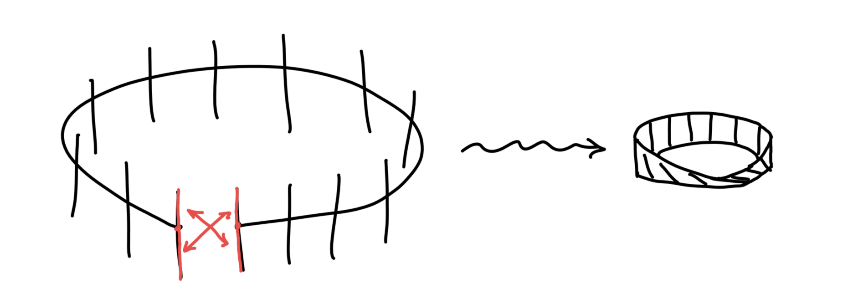
\includegraphics[scale=0.4]{chern_mobius1}
\end{figure}
\begin{exercise}
    Check that this defines a vector bundle, by seeing that on an actual open
    cover of $S^1$ we have local trivializations and transition maps, as in the
    following figure.
\end{exercise}
\begin{figure}[htb]
    \centering
    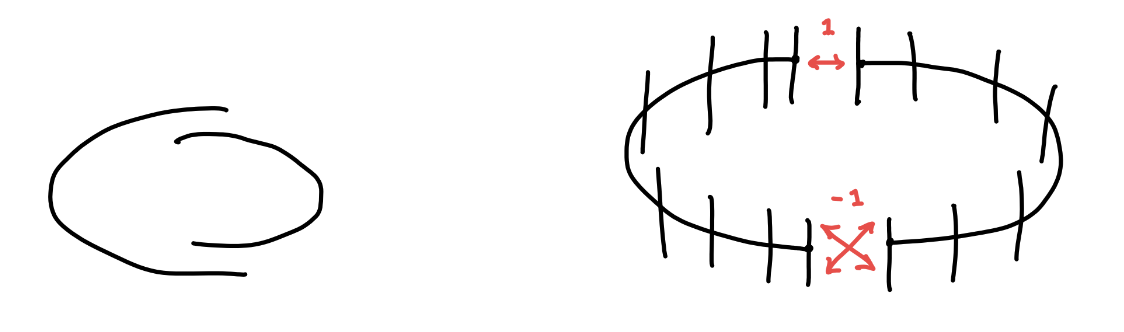
\includegraphics[scale=0.3]{chern_mobius2}
\end{figure}
\begin{exercise}
    If instead of one twist we include two twists, show that the resulting
    bundle is trivial. Further, show that it can be untwisted to the standard
    band if embedded in $\R^4$.
\end{exercise}

\paragraph{Exercises.} So we may think of $E$ as $\coprod_U(U\times\C^r)/\sim$,
where we glue by the transition functions $g_{UV}$; for $x\in U\cap V$ we
identify
\begin{equation*}
    V\times\C^r\ni(x,e) \sim (x,g_{UV}(x)e)\in U\times\C^r.
\end{equation*}
\begin{exercise}
    Check that this defines an equivalence relation, and that the quotient is
    $E$.
\end{exercise}
\begin{exercise}
    Show that the fibres of $\pi$ are naturally vector spaces: if $x_1=(x,e_1)$
    and $x_2=(x,e_2)$ are points of the same fibre $E_x=\pi^{-1}(x)$ and
    $\alpha,\beta\in\C$ we can define $\alpha x_1+\beta x_2\in E_x$ such that...
\end{exercise}
\begin{exercise}
    Define smooth vector bundles over a smooth manifold, algebraic vector
    bundles over algebraic varieties, real vector bundles, e.t.c.
\end{exercise}

\paragraph{Sections.} A section of $\pi:E\to X$ is a continuous map $s:X\to E$
such that $\pi\circ s=\id_X$. They form a vector space $\Gamma(E)$ by the
fibre-wise vector space operations.
\begin{exercise}
    A trivialization of the bundle, i.e. an isomorphism
    \begin{equation*}
        \begin{tikzcd}
            &E \ar[d,"\pi"] \ar[r,"\sim"]
                &X\times\C^r \ar[d,"{(x,v)\mapsto x}"] \\
            &X \ar[r,equals] &X
        \end{tikzcd}
    \end{equation*}
    is the same thing as a choice of $r$ sections $s_1,\ldots,s_r$ which form a
    basis at every point, i.e. $s_1(x),\ldots,s_r(x)$ is a basis of $E_x$ for
    every $x\in X$. Hence a trivialization of a line bundle is the same thing as
    a nowhere-vanishing section.
\end{exercise}

\paragraph{Homotopy invariance.} We have
\begin{itemize}
    \item \textbf{Fact 1:} Homotopic bundles are isomorphic. Given
        $E\to X\times[0,1]$, writing $E_t=E|_{X\times\{t\}}$ we have
        $E_0\cong E_1$.

    \item \textbf{Fact 2:} Bundles on contractible spaces $X$ are trivial. If
        $X\simeq\{*\}$ then any bundle $E\to X$ is isomorphic to $X\times\C^r$.
\end{itemize}
For proofs using the Tietze extension theorem see Atiyah's \emph{$K$-Theory}.

So given a rank $r$ bundle $E\to S^n$, we know that restricted to either
hemisphere it is trivial,
\begin{equation*}
    S^n = B^n_1\cup B^n_2, \qquad E|_{B^n_i}\cong B^n_i\times\C^r.
\end{equation*}
These restrictions are glued over the boundary $\partial B^n_i\cong S^{n-1}$ by
a map $S^{n-1}\to\GL(r,\C)$. (Strictly speaking we should take slightly larger
open hemispheres, intersecting in an open annulus which contracts to this
boundary.)

\paragraph{Clutching construction.}

\end{document}
